% !TeX spellcheck = en_GB
% !TeX encoding = UTF-8
% !TeX root = mosaicStitching.tex

\section{Image Stitching}
\label{sec:ImageStitching}
A logical method to create a full digital plan from the photomotric stereo outputs is to stitch them together in a manner similar to that used when creating panorama images. As the ability to automatically stitch together images has existed for some years now - including panoramic functions in mobile phones - an existing software solution was sought to automatically combine the patches into a full Plan. For most stitching software, they generally implement the following steps:
\begin{enumerate}[nosep]
	\label{}
	\item Feature Detection and Matching
	\item Extrinsic Camera Paremeter Optimisation
	\item Seam Determination and Blending
\end{enumerate}

Due to the methodology incorporated for the photometric stereo captures, some further assumptions could be made about the relationship between patches to help existing software obtain an optimal solution. By having the camera approximately orthogonal to the Plan and shifting the trolley underneath the camera, this enables the assumption that extrinisic camera parameters determined would consist solely of translations in the XY plane and a rotation around this Z axis (represented as the camera viewing direction) - also seen as a 2D rigid transformation in 3D space.

On the other hand, there were additional requirements and desired functionality of the stitching software to ensure  optimal results. Firstly, as each data acquisition of the plan using the white light and multispectral produced normal, ambient and albedo maps, it was desired that the software could produce a single set of extrinsic camera parameters for each of the MiniDome acquisitions. As all the normal, ambient and albedo maps are determined from the same set of images captured by the MiniDome and their pixels corresponding to the same surface area of the plan, it was important that the same set of extrinsic parameters should define the transformations for all output formats. This helps ensure that the pixels in each stitched Plan have correspondence across the different output formats. This is equally important for the multispectral acquisition where the three output formats were produced for each of the five wavelengths observed by the multispectral camera. Without this pixel correspondence, the multispectral outputs are not easily comparable on a full Plan scale with reliable results obtained only on a patch-by-patch basis.

In the end, four different software were tested to try and create a fully stitched Plan from the output products. These consisted of Photoshop, Image Composite Editor (ICE), Huginand OpenCv. Although only three of these software were succesfully used to create a fullly stitched Plan from the full resolution patches, each will be discussed in terms of their functionality, suitability and quality of results from those that were successful.

\subsection{Hugin}
\label{sec:Hugin}
Hugin is an open source panorama stitcher based on the Panorama Tools suite \cite{Hugin2019}. The software is based around panoramic stitching which bases itself on a centrally positioned camera with a rotating perspective, it does have the capability to accommodate translations of the camera with respect to the resulting stitched panorama.

One of the key advantages of this software falls largely in it being open source. Because of this, there is a large varietz of functionality and control of the whole stitching process. This ranges from controlling the featured matching and seam blending functions, to selecting which transformation parameters to optimise between the overlapping, to ultimately being able to output textfiles containing the whole set of project parameters that entail the stitching process.

	\myparagraph{Key Point Extraction}
	The Hugin software allowed for a variety of different feature detection algorithms to be used for identifying control points which would be used for the determination of relative orientation parameters. This is a two step process, the first of which discussed here, is the creation of keypoints. This keypoint creation is also a two step process. First a generic feature detection algorithm is run across the whole image, creating a comprehensive set of features for each image. The next step involves subsampling these features across the image. All the features are binned into cells of an equally spaced grid and the most unique features within each cell of the grid are taken to be used as the keypoints from the image which will be matched with those from other images. The number of rows, columns and unique features per cell can all be defined by the user to help control the distribution or number of features to be matched. Improvements to the matching process can be gained through this process by increasing the number of features, and thus the number of matches, or reducing the number of features to be compared in the matching and in turn reducing the processing time required.

	An issue was identified with the keypoint generation on the normal maps though. This was because as the normal maps provided a representation of geometric properties within an image's colour channels. For very planar and continous regions, this presents similarly to areas of uniform colour in a truecolour image and not showing the distinct photometric properties that are ideal for detecting features. This in turn left large areas within the normal maps free from detected features. This become a problem as there was not a good distribution of keypoint for the matching algorithm with which the external camera orientation parameters would be determined from and could bias the results. 
	
	\myparagraph{Control Point matching}
	Once a full set of keypoints was acquired for each of the images, the second part of the control point generation involved firstly searching for matches with all other keypoints from the other images. Once matches were identified between images, similarly to the keypoint detection, a subsampling grid would be used to further reduce the number of matched keypoints that would become the control points tieing the images together and basis for determining the homographies between the images to create the stitched plan. This subsampling greatly reduced the number of matched control points whilst maintaining a good distribution to help ensure that the optimisation was performed efficiently. 
	
	As mentioned before, the there were often large gaps in the overlapping regions of the normal maps that were matched. Since all the pixels in the normal, ambient and albedo map correspond to each other, the geometric relation between matched keypoints from each image should be identical. Based on this assumption, matched control points from both ambient images and normal maps were combined for each stitched Plan. Doing this helped ensure that there was a good distribution of control points across the overlapping regions for which the image transformation parameters would be determined. Control points from th albedo were not included as there appeared to be a negligible improvement in the results for the considerable increase in processing time.
	
	\begin{figure}[H]
		\centering
		\begin{subfigure}[b]{1\textwidth}
			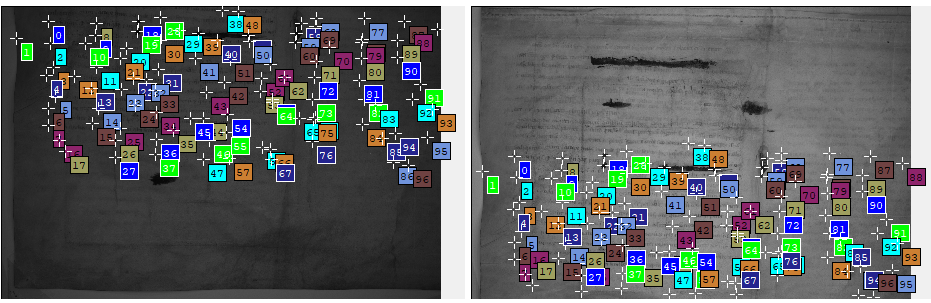
\includegraphics[width=1\linewidth]{img/AmbientFeatures.PNG}
			\caption{}
			\label{fig:AmbientFeatures} 
		\end{subfigure}
		
		\begin{subfigure}[b]{1\textwidth}
			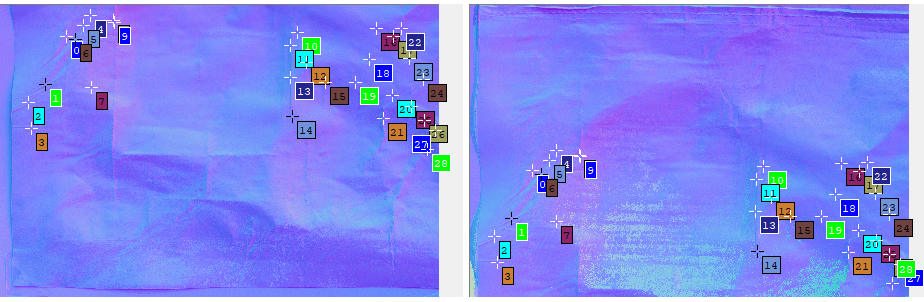
\includegraphics[width=1\linewidth]{img/NormalFeatures.PNG}
			\caption{}
			\label{fig:NormalFeatures}
		\end{subfigure}
	
		\begin{subfigure}[c]{1\textwidth}
			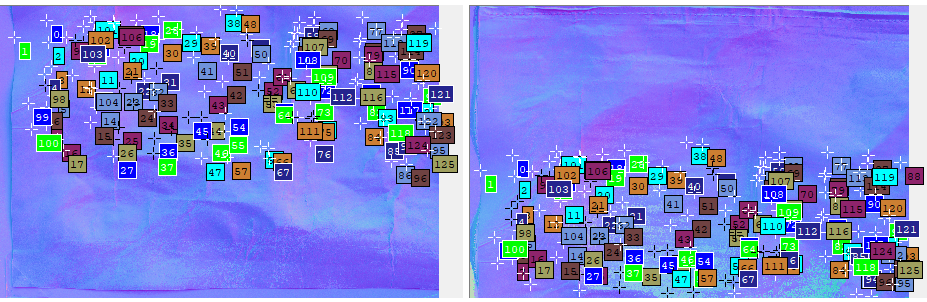
\includegraphics[width=1\linewidth]{img/CombinedNormalFeatures.PNG}
			\caption{}
			\label{fig:CombinedFeatures}
		\end{subfigure}
		
		\caption[Comparison of Control Point Matches]{(a) Control points matched between the ambient images, (b) sparse distribution of control points matched from the same normal maps and (c) the final combined set of matched control points. }
	\end{figure}

	\myparagraph{Control Line Creation}
	One of the key constraints on the stitching of the Plan in Hugin to ensure the best results was in creating some vertical and horizontal control lines along the edges of the carton the plan was held in. By doing this, it provided references in the software that would constrain the parameters such that the stitching of the plan within a rectilinear projection would stay straight. This helped act as a boundary condition to maintain the external shape of the stitched plan whilst there was sufficient overlap internally to ensure a good alignment was found of the internal patches.
	
	\begin{figure}[H]
		\centering
		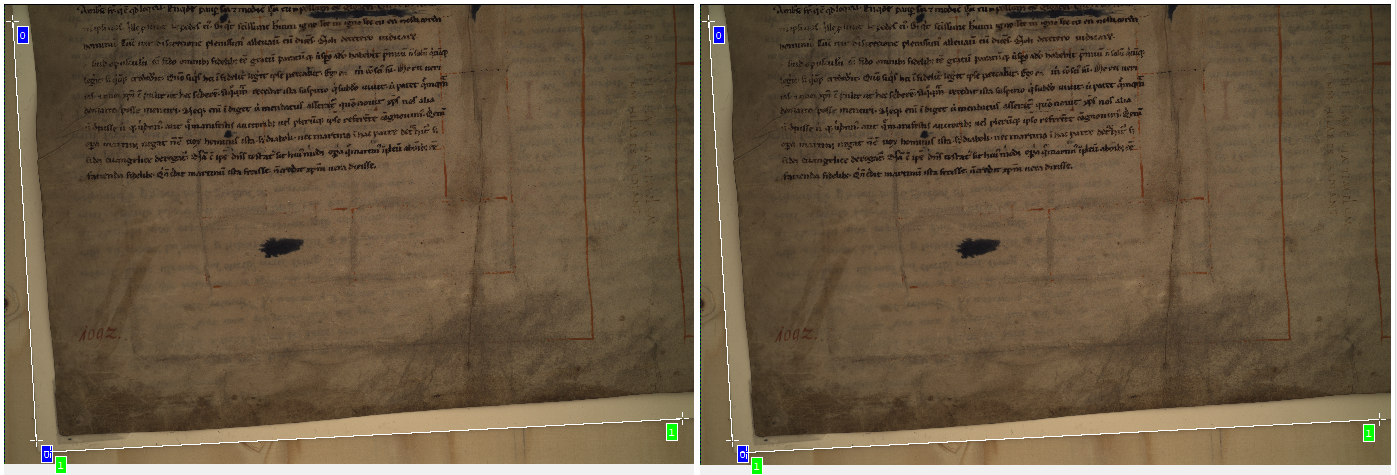
\includegraphics[width=1\textwidth]{img/ControlLines.PNG}
		\caption{Example of the control lines marked on the edge of the cardboard the Plan is held on.}
		\label{fig:ControlLines}
	\end{figure}
	
	\myparagraph{Extrinsic Parameter Optimisation}
	As stated in \cref{sec:ImageStitching}, it was assumed that the relative camera motions of translations in the XY axes and a rotation around the Z axis would reasonably represent the relative motions of the trolley with respect to the camera. For the final output, these parameters were the only ones optimised for each of the images within the Hugin software. Additional parameters available such as plane pitch and yaw and camera rotations around the X and Y axes were applied to all images from the optimised solution to ensure that the control lines created along the cardboards edge remained straight. This helped correct a slight perspective distortion of the plan that arose from the camera not being perfectly orthogonal to the trolley plane.
	
	\begin{figure}[H]
		\centering
		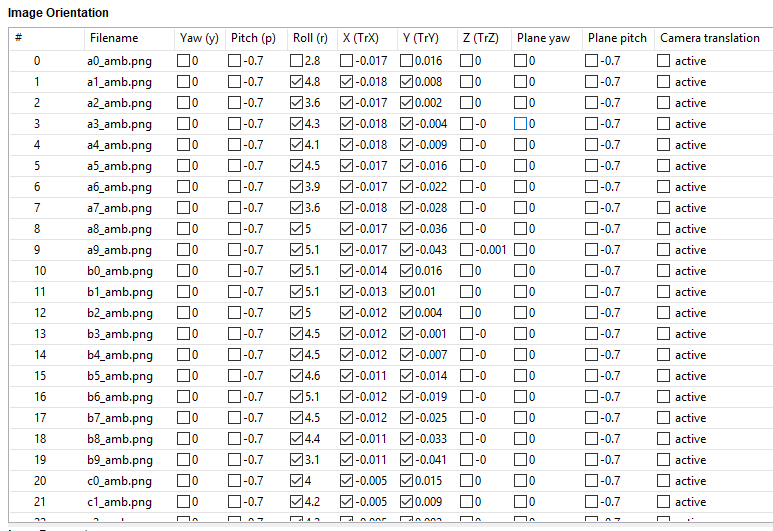
\includegraphics[width=1\textwidth]{img/HuginOrientationParams.PNG}
		\caption{Example of the interface for the extrinsic camera parameter optimisation and the determination of unique XY translations and Z (roll) rotations of the images.}
		\label{fig:OrientationParams}
	\end{figure}
	
	\myparagraph{Intrinsic Parameter Optimisation}
	Hugin is also capable of determining the intrinsic camera calibration parameters for removing image distortions caused by a typical pinhole camera model. For this project though, these parameters were kept set to zero as attempts to determine these parameters in addition often lead to an unconstrained solution and significant issues in the final stitched plans. Had the determined intrinsic parameters been provided by the group at ESAT, these could have been entered into Hugin and helped improve the results.
	
	\myparagraph{Photometric Correction}
	In addition to the determination of the extrinsic camera paremetes relating all of the patches to the plan, photometric corrections could be determined through the software to improve the photometric blending across the full plan. For the stitched results using Hugin, no exposure or photometric corrections were determined or applied to the individual patches as precise corrections were determined for the exposure and vignetting effects of the images in the ESAT processing to output the normal, ambient and albedo maps.
	
	\myparagraph{Plan Preview}
	One of the most useful features of the Hugin software was the preview function shown in \cref{fig:HuginPlanPreview}. This enabled the user to try different sets of transformation parameters and perform a sanity check on the results before submitting it to be processed in the batch processor. A cropping tool also helped in trimming the output Plan to ensure that there were no blank pixels and minimise the extra area surrounding the plan to be included in the stitched image.
	
	\begin{figure}[ht]
		\centering
		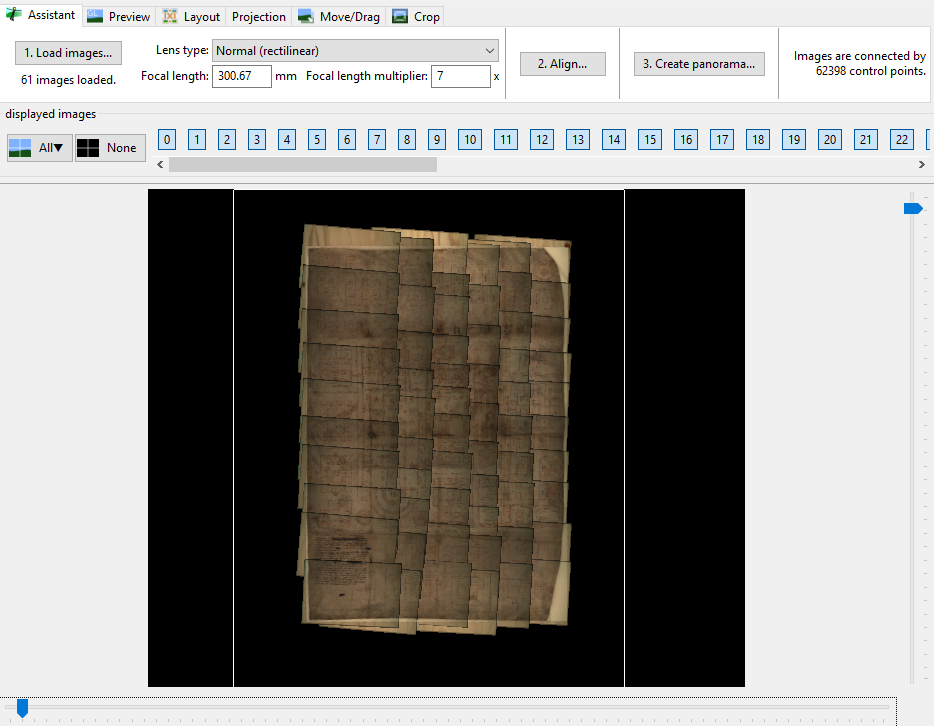
\includegraphics[width=1\textwidth]{img/Hugin_Preview.PNG}
		\caption{Example of the stitching preview in Hugin}
		\label{fig:HuginPlanPreview}
	\end{figure}
	
	\myparagraph{Batch Processing}
	Finally all the stitching projects created in Hugin are stored in a text file. All the parameters that were optimised, control points that are matched and final stitching processes to be performed are all recorded within this text file. Because of this, once a set of control points were identified for the white light and multispectral acquisition, only a single set of transformation parameters were required to be optimised for each acquisition. As these were easily linked to the associated image patch within the project text file, it was simple to copy the project file and change paths of the images for each output format or wavelength so that each stitched Plan per output and wavelength used identical transformation parameters for each of the acquisitions.
	
	Furthermore, as the Hugin had batch processing capability, this allowed all the different project text files to be aded to the queue and reduce the manual workflow required to produce all stitched Plans.
	
	The final outputs from the Hugin processing will be shown in \cref{sec:ResultsStitching} and discussed further in \cref{sec:DiscussionStitching}.

\subsection{Photoshop}
\label{sec:Photoshop}
Unlike Hugin, Photoshop is a proprietary piece of software that requires a paid license to utilise. Within the software suite it contains a function called "Photomerge" which allows for the automatic stitching of the plan. The number of parameters that the user could control with regards to the stitching process were minimal, consisting of the simple selection of a projection model and then a couple parameters regarding the option of exposure and geometric distortion correction. 

As the rest of the software produced a closed box solution, each set of output or wavelength images passed into the Photomerge function would produce a slightly different result as the feature detection and transformation parameter processed is unique to the input set of images. Although the results might be similar in dimension, it is hard to say that the pixels in one stitched plan correspond to those in another which is not ideal for analytical purposes. 

One of the benefits of creating the Plans using Photoshop was the ability to output the remapped images for the stitched Plan. Although the transformation parameters were not output specifically, one could perform a feature detection and matching between the remapped layer and the original image to determine the homography between them and obtain a full set of homographies that define the transformation of the input patches to the stitched outputs. The seams determined in Photoshop could be acquired as image masks were also attached to the output layers which showed the region that was included in the final mosaic. It is not exactly clear if there was blending of the pixels along the seams but it made it easy to output clipped overlapping regions and perform a comparison with the mosaic. This helped to perform a statistical analysis of the quality of stitching. 

Again, see \cref{sec:ResultsStitching} for some of the results pertaining to the Photoshop processing and \cref{sec:DiscussionStitching} for further analysis of them.

\subsection{Image Composite Editor - ICE}
\label{sec:Ice}
ICE is a freely provided software by the Microsoft Research group but is more similar to Photoshop in its closed box solution and limited ability to control the stitching workflow. In comparison to Photoshop though, it does have a few more parameters to help with the stitching process.

Firstly, there are more projection options available with ICE including a perspective projection. This is most representative of the projection model most suited to the stitching of the Plan compared to other projections offered in Hugin. Although it is assumed that the camera of the Minidome is orthogonal to the trolley plane, there is likely a slight misalignment, thus a perspective reprojection would allow for a little bit of freedom given any errors in the angle intersected by the camera line-of-sight and the trolley plane.

Another useful aspect of the software was the definition of "structured panoramas" where an equally spaced grid of images is taken to be stitched together. One problem with this though was that the number of rows and columns set, so the number of images per column is fixed. Thus for the white light acquisition, the third column captured 11 images across the plan whereas all the others captured 10, so this function could not be used. For the multispectral acquisition it could be implemented though as there were an equal number of images captured along each column across the plan. It also allowed the approximation of the overlap between images in horizontal and vertical directions to help define a good starting a priori for the full stitching process.

By using this "structured panorama" functionality, reasonably nice results were acquired and exceptionally quick compared to all other stitching software tested. Only some test plans were generated from ICE though as there were no intermediate outputs and no ability to constrain the patch transformations with respect to each Minidome capture making it difficult for reliable analysis across stitched outputs.

\subsection{OpenCV}
\label{sec:OpenCv}
OpenCV was an instinctive option for attempting to stitch the Plan of St Gall from the individual patches with its wide range of Computer Vision algorithms. One of the algorithms was a high level stitching API provided within the software \cite{OpenCV2019}. Promising aspects of the OpenCV software was the ability to control different parameters in the stitching process via a method to replicate a scanner or drone captures where there is an affine transformation between the images as compared to homographies. Attempts to immplement the stitcher in its scanner or panorama methods using the built in class or the \texttt{detailed\_stitcher.py} function.

Attempts in using the stitching class had mixed results but were not proving to be successful on the full resolution data... Infinite loop or exceptionally long processing time?

Because no results were being obtained for the full resolution datasets, this pathway was abandoned but the stitching class had some functionality and ability to output all determined parameters and intermediate results which would have been of interest for this project. In particular, fine tuning the fully stitched Plan, but also analysing the quality of results.

\subsection{Wavelength Differences}
As the multispectral Minidome acquisition produced normal, ambient and albedo maps for all five wavelengths captured, one point of interest for investigation will be in the differences between the data captured in each wavelength. As absolute and directional differences between the various wavelength combinations were produced on a patch by patch basis for all output products, these difference products could also be combined into stitched Plans for easier investigation of the variations between wavelengths across the whole plan.

\subsection{Overlap Differences}
Sufficient overlap between the patches were acquired to ensure that a full stitching of the Plan could be performed from the photometric stereo survey. Unfortunately, the parchment's geometric surface can change slightly over time due changes
in humidity which would mean the surface of the plan could differ between each acquisition epoch. As the patches were acquired column-by-column along the plan, little differences is expected to be seen due to only a couple of minutes of time pass between the neighbouring patches along the same column. Difference in the overlapping regions could potentially be greater in the neighbouring columns as the time between patches is considerably longer and be close to an hour in most cases or even longer for breaks taken during each acquisition.

By taking the difference in the normal maps in the overlapping regions, there is potential to observe this "breathing" effect of the plan as it curls due to changes in humidity. To do so, the remapped image patches used to generate the stitched plans from Hugin were taken and the absolute and directional differences in the overlapping areas of the normal maps were taken to attempt to identify this elastic deformation of the Plan.

\subsection{Results}
\label{sec:ResultsStitching}

\subsubsection{Hugin}

\subsubsection{Photoshop}

\subsubsection{ICE}

\subsubsection{OpenCV}

\subsubsection{Wavelength Differences}

\subsubsection{Statistical Comparison}

\subsubsection{Homography Determination}

- Photoshop provided some of the most visually appealing results.
- Line work and visual features were nearly all continuous with minimal discontinuities compared to others
- Hugin could be consistent with the remapping and projection of results
- Line control points provided additional constraints to the outside of the plan to ensure they were "straight" and not so affected by projective distortions
- Ice was extremely fast and easy... although issues with the layout option for the white light as the software was rigid that all row and columns must contain the same number of images
- Results were visually appealing... Equal with photoshop?

\subsection{Analysis and Discussion}
\label{sec:DiscussionStitching}

	\subsubsection{Fully Stitched Plan Quality}
	\label{sec:PlanQuality}
	In terms of the quality of stitching it is hard to distinctly say which is the best or better in terms of results. This all depends on what the final stitched Plan is being used for. One point of comparison is the visual continuity of the features on the Plan. For example, lines on the plan continue through all patches and are not broken where the seams were computed and blended. Minimisation of projective distortions was also one point of comparison as some geometric properties of the plan are broken.
	
	In terms of visual continuity it appears that the results from Photoshop's 'Auto' option produced were arguably the best. There appeared fewer and less obvious discontinuities in the line work compared to that output by Hugin. The choice to use the geometric distortion correction or not yielded varying results. In some cases it reduced the projective distortions but in others it appeared to be worse. These projective distortions were significantly more noticeable than compared to the Hugin results as shown in FIGURE X.
	
	The results from ICE also produced some visually appealing results like Photoshop but the ability to use a perspective projection helped maintain the geometric shape of the plan similarly to Hugin. Additionally, the result from ICE was produced significantly quicker but the speed of production is not a serious consideration


- Errors in the stitching

- Comparison of the reprojection

- Comparison of the quality of seam blending

- Differencing of the plan

- Observation of the elastic deformation of the plan throughout the iterative process

